\chapter{Analisis de los resultados}

En este capitulo se analiza varios aspectos de la tecnica digital en contraste con la tecnica tradicional buscando validar la solucion propuesta y demostrar las ventajas que esta presenta. \\ 

\section{Comparacion de perfiles}
Utilizando los resultados presentados en los ensayos \ref{sec:ensayo-erosion-maxima}, se comparan perfiles obtenidos con ambas tecnicas con el objetivo de estudiar la bondad de la tecnica digital para relevar la condicion de erosion. \\
En la figura \ref{fig:comparacion-perfiles}, se muestran tres perfiles sobre el foso de erosion capturados con las tecnicas digital y tradicional.\\

\begin{figure}[ht]
\centering
\begin{minipage}[h]{.45\textwidth}
\begin{center}
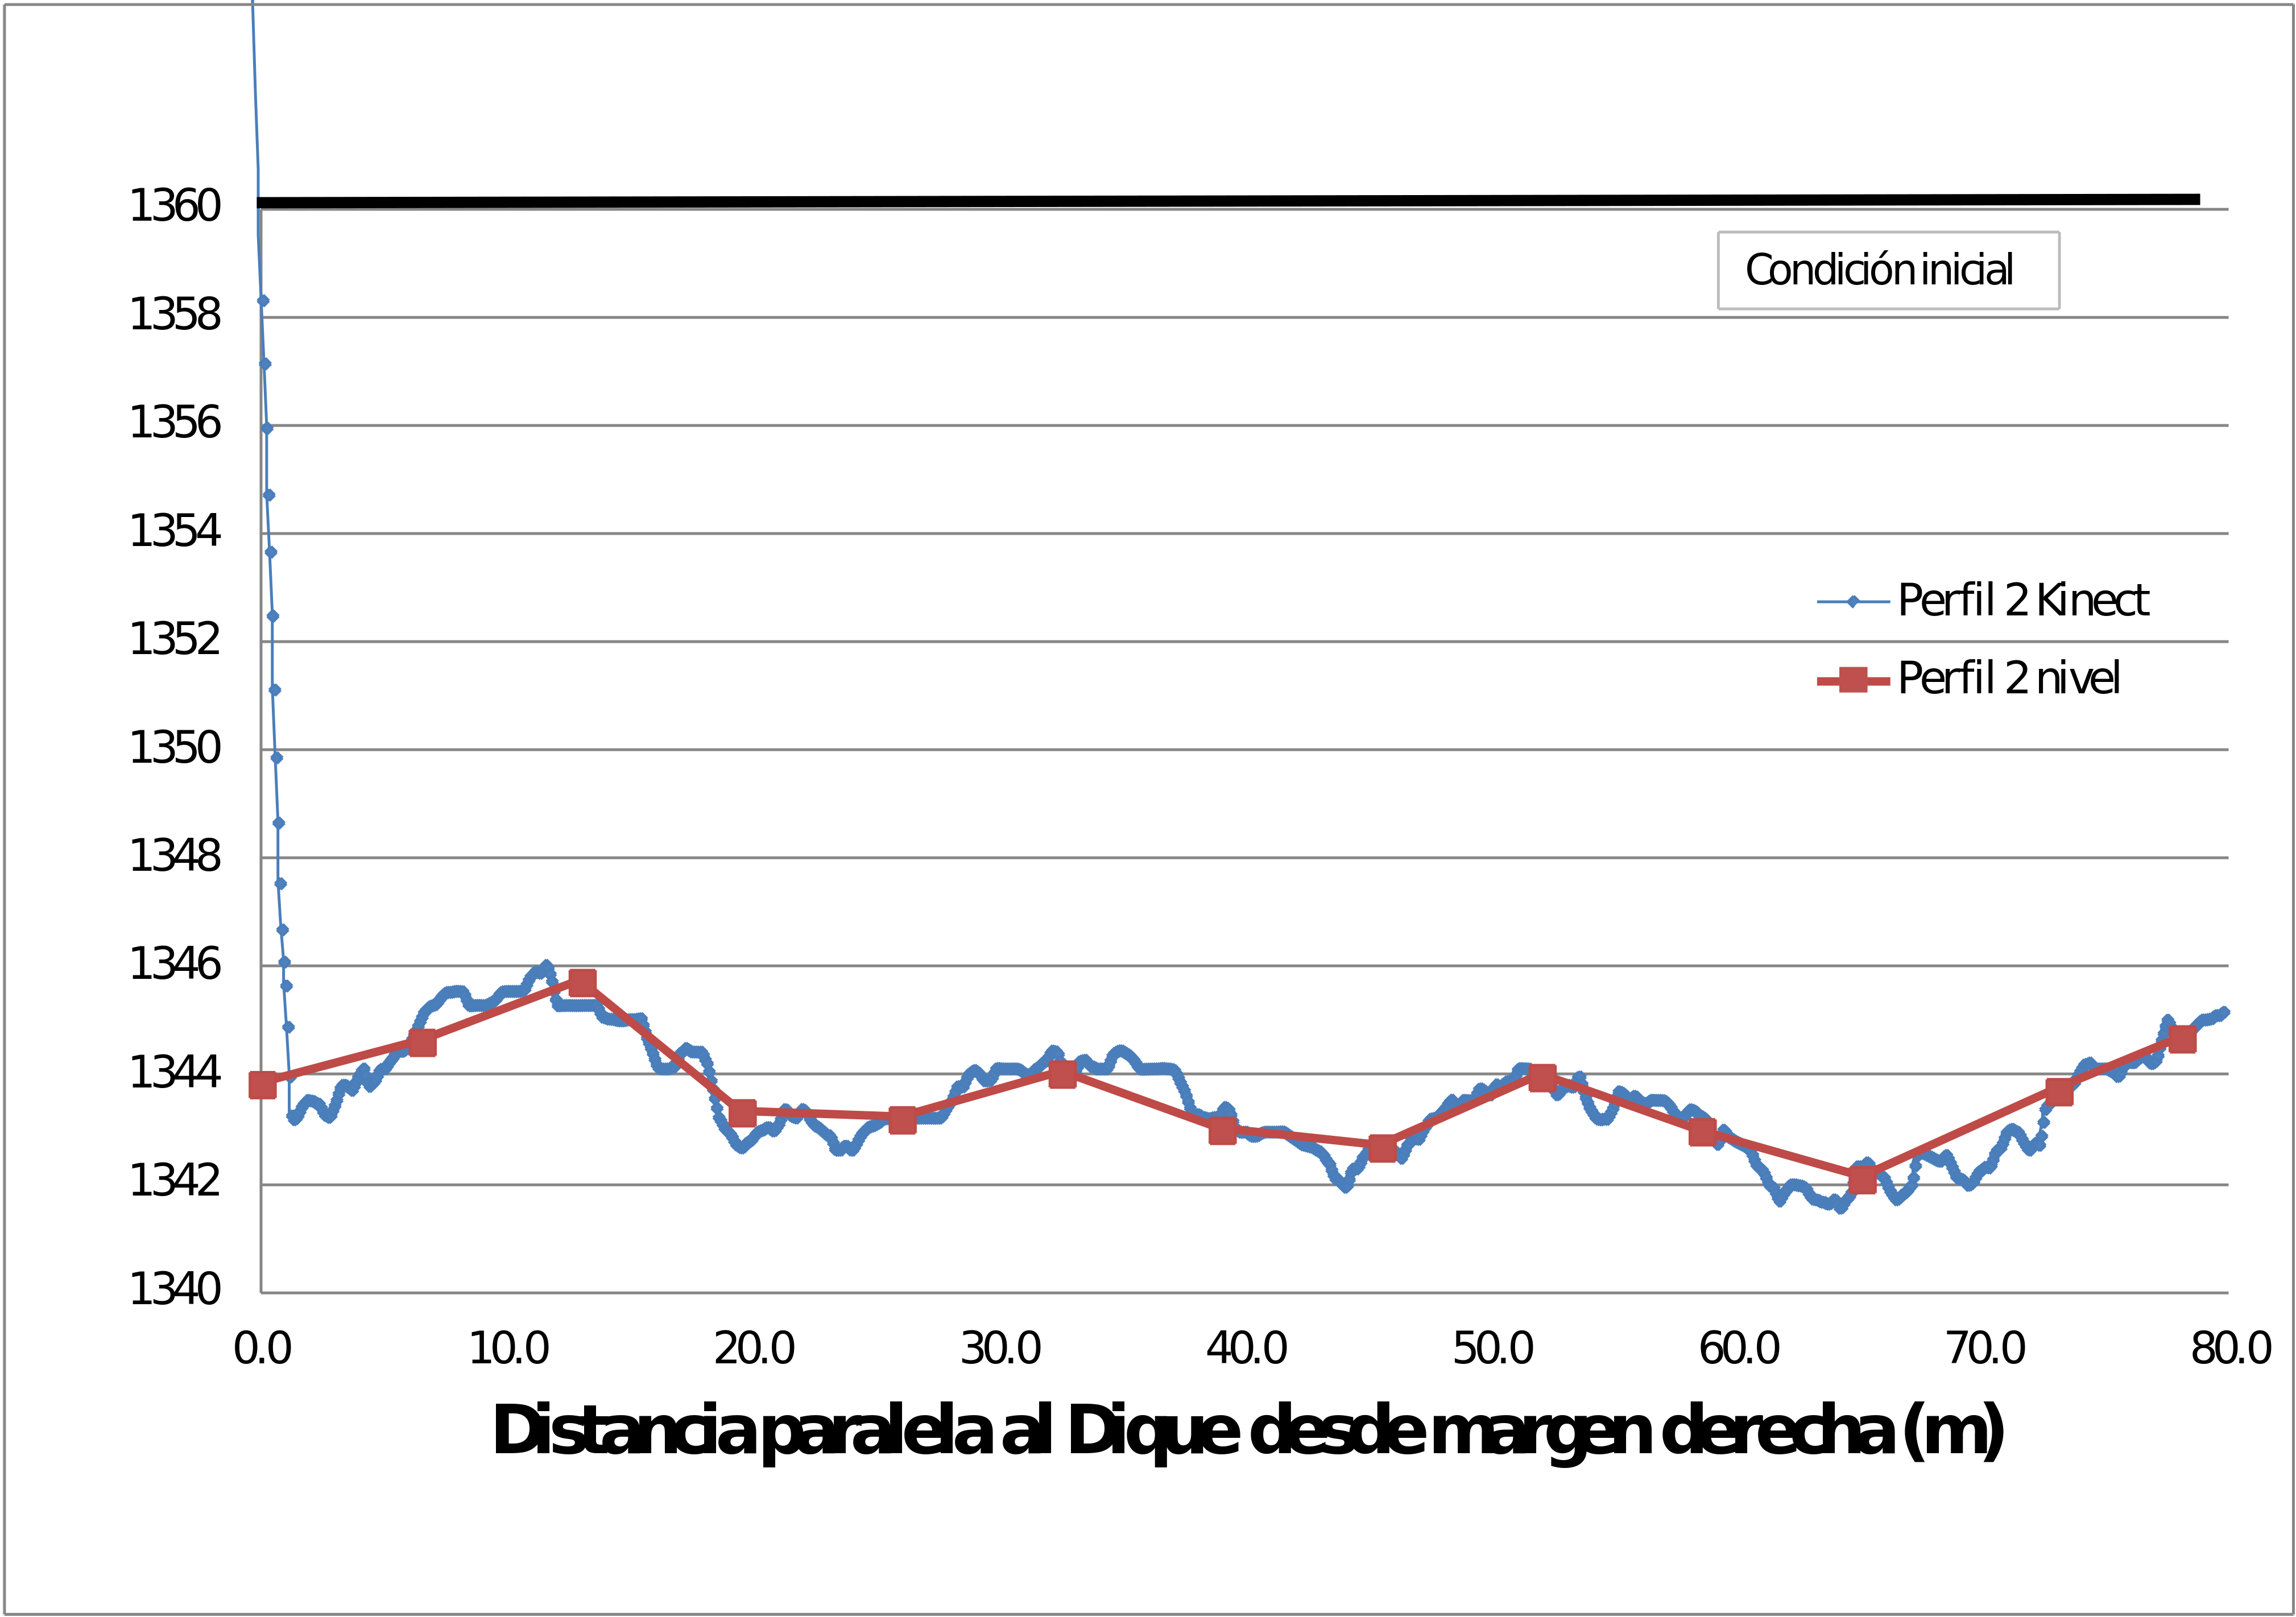
\includegraphics[width=\imsizeS]{foso-erosion-izquierda}
\end{center}
\end{minipage}
\hfill
\begin{minipage}[h]{.45\textwidth}
\begin{center}
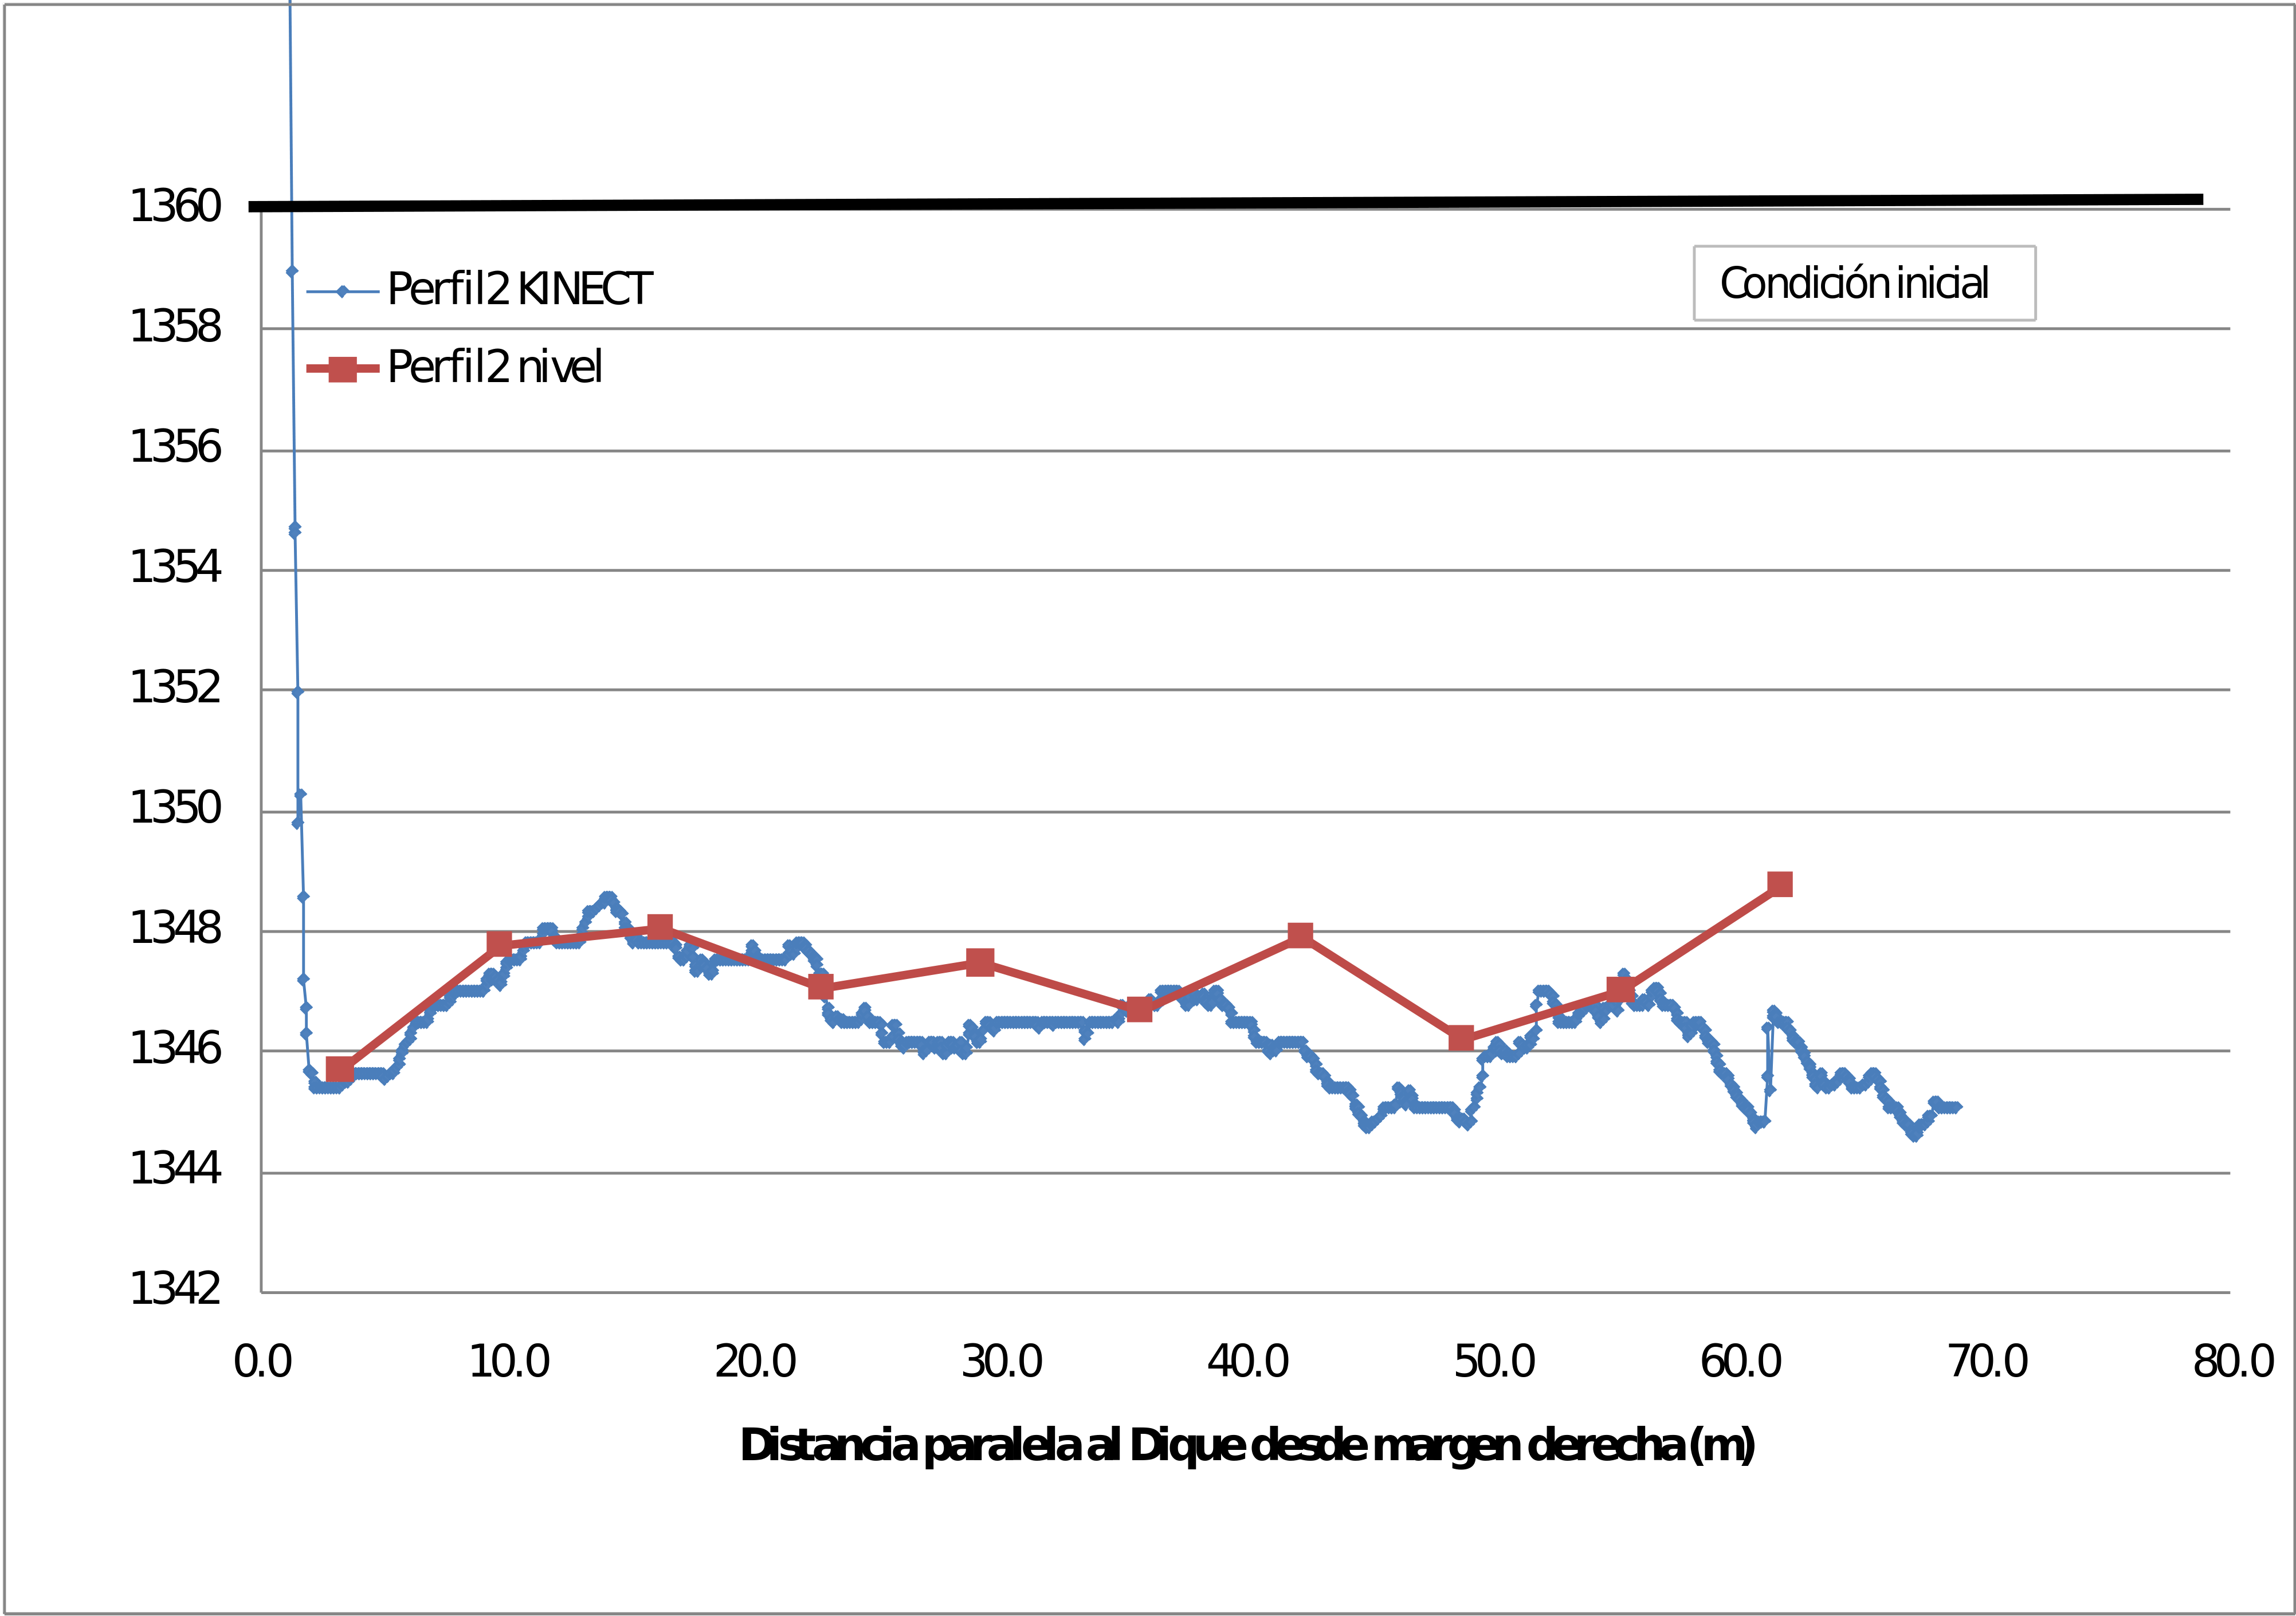
\includegraphics[width=\imsizeS]{foso-erosion-centro}
\end{center}
\end{minipage}
\hfill
\begin{minipage}[h]{.45\textwidth}
\begin{center}
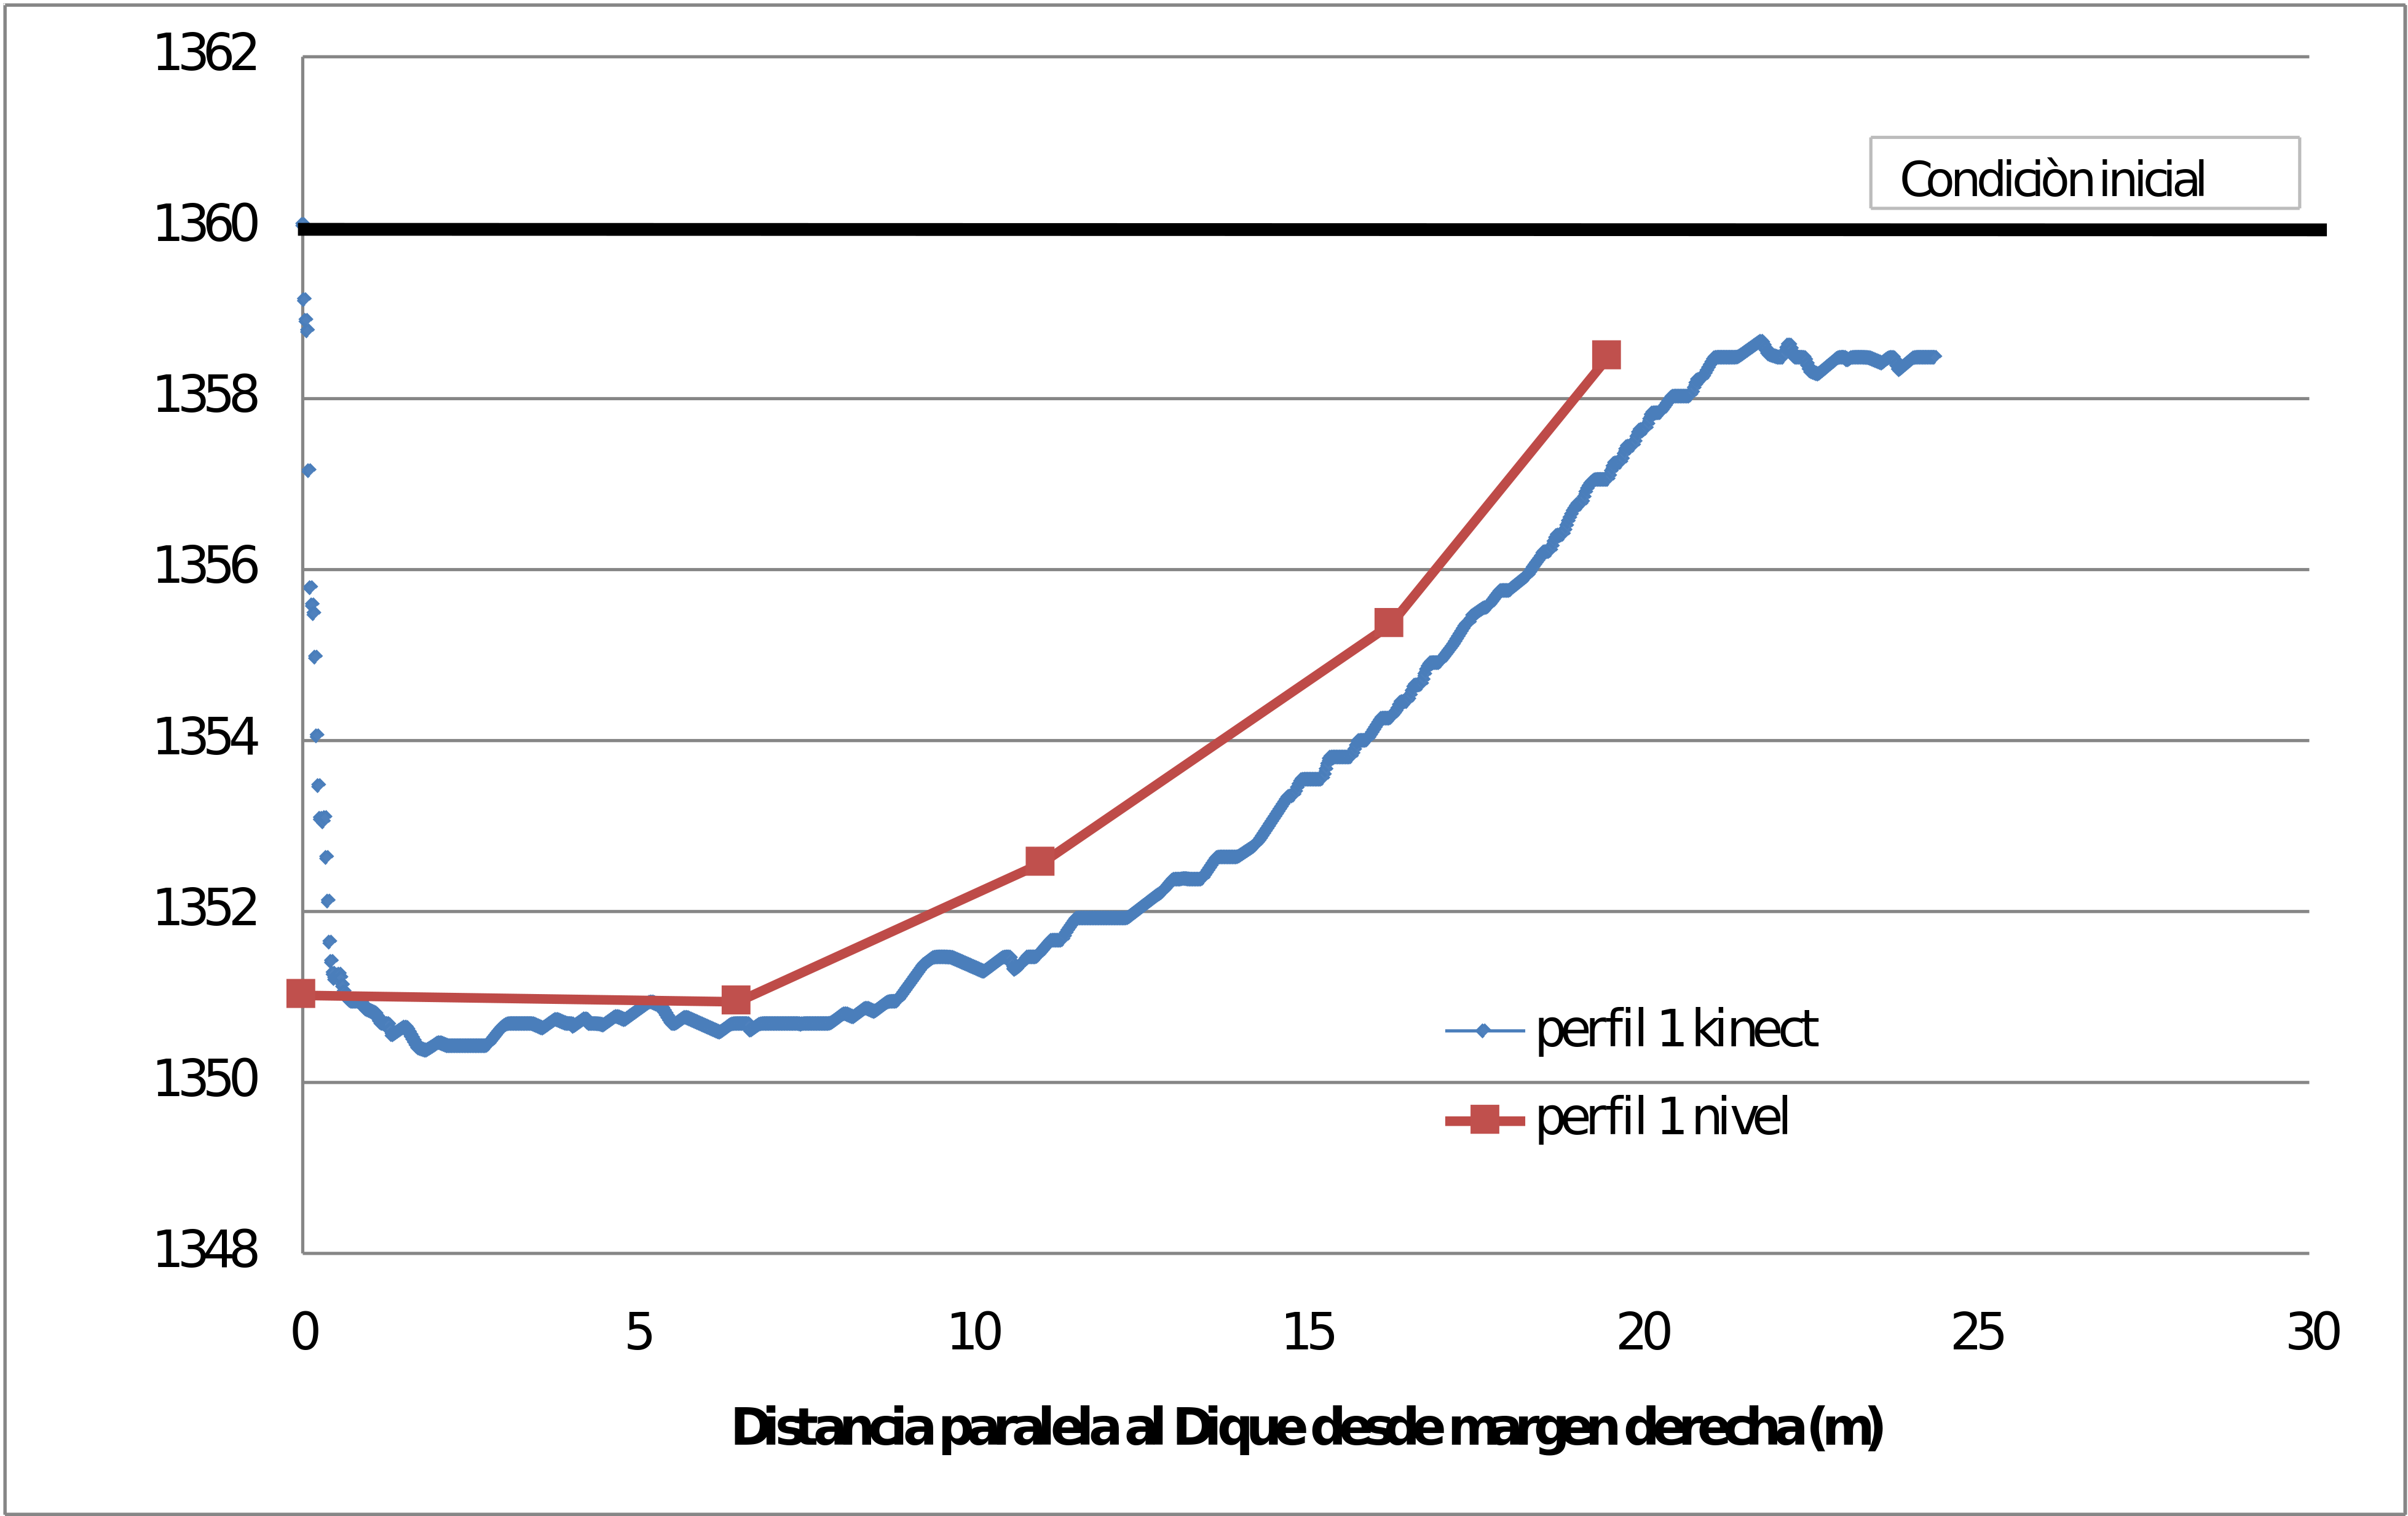
\includegraphics[width=\imsizeS]{foso-erosion-derecha}
\end{center}
\end{minipage}
\hfill
\caption[Perfiles foso de erosion]
{Perfiles foso de erosion}
\label{fig:comparacion-perfiles}
\end{figure}

En el perfil superior izquierdo, se observa que los datos continuos relevados con la camara son aproximados de forma precisa por las mediciones con nivel optico en condiciones donde el terreno no presenta cambios abruptos. \\
En el perfil superior derecho, se observan 3 mediciones, a 30 m, 42 m y 60 m respectivamante, que se presumen haber sido tomadas de forma incorrecta con el nivel optico. No obstante, sirve para ilustrar que la tecnica tradicional puede sufrir de errores de hasta 15 mm en prototipo, o equivalentemente, 1 m en prototipo (utilizando una escala 1:65) que no podrian ser detectados sin una superficie de referencia. Aproximadamente a los 50 m se incurre en un error de una indole distinta. En este caso, la causa de la medicion incorrecta es un cambio abrupto en la condicion del terreno, que no pudo ser detectada por el operador de la mira debido la escala del modelo. \\ 
En ultima instancia, se presenta el perfil inferior donde se observa el efecto de la pendiente del foso de erosion sobre una serie de mediciones con nivel. En este caso, la pendiente dificulta el apoyo del palpador sobre la superficie sin producir alteraciones, derivando en mediciones por encima del valor real. \\
Estas comparaciones ponen en evidencia que la resolucion del modelo 3D obtenido con la tecnica digital, es superior en zonas donde los datos relevados con la tecnica tradicional no han sido cuidadosamente elegidos o el terreno es muy irregular. Cuando estos errores no estan presentes, la precision de ambas tecnicas se encuentra similar.

\section{Erosion maxima}

A continuación se presentan las máximas erosiones observadas en el foso de erosión aguas abajo del canal moderador y el dique móvil relevando tanto con nivel y mira como con la cámara RGB-D.

\begin {table}[H]
\caption {Máximos niveles de erosión en el Canal Moderador} 
\label{tab:erosion-maxima-cm} 
\begin{center}

\begin{tabular}{|c|c|c|c|c|}
\hline 
Caudal  $m^{3}/s$ & Ensayo & Nivel optico (m) & Kinect  (m) & Diferencias absolutas (m) \\ 
\hline 
90 & 4 & 1350.96 & 1350.37 & 0.59 \\ 
\hline 
600 & 14 & 1349.5 & 1349.16 & 0.34 \\ 
\hline 
900 & 1 & 1344.8 & 1345.75 & 0.95 \\ 
\hline 
1600 & 13 & 1345.7 & 1345.38 & 0.32 \\ 
\hline 
4200 & 7 & 1345.2 & 1345.59 & 0.39 \\ 
\hline 
4200 & 9 & \textbf{1344.6} & \textbf{1344.18} & 0.42 \\ 
\hline 
     &   &        & Promedio & 0.498 \\
\hline 
\end{tabular}
\end{center}
\end{table}

\begin {table}[H]
\caption {Máximos niveles de erosión en el Dique Móvil} 
\label{tab:erosion-maxima-dm}
\begin{center}
 
\begin{tabular}{|c|c|c|c|c|}
\hline 
Caudal  $m^{3}/s$ & Ensayo & Nivel optico (m) & Kinect  (m) & Diferencias absolutas (m) \\ 
\hline 
220 & 5 & 1354.2 & 1354.89 & 0.69 \\ 
\hline 
600 & 14 & 1350.1 & 1349.67 & 0.43 \\   
\hline 
900 & 1 & 1346.1 & 1345.86 & 0.24 \\ 
\hline 
1600 & 13 & 1346.2 & 1344.56 & 1.64 \\ 
\hline 
4200 & 7 & \textbf{1342.3} & \textbf{1343.2} & 0.9 \\  
\hline 
4200 & 9 & 1343.2 & 1343.41 & 0.21 \\ 
\hline 
     &   &        & Promedio & 0.685 \\
\hline 
\end{tabular}
\end{center}
\end{table}

NO SE QUE CONCLUIR CON LOS PROMEDIOS

ENSAYO Q1600 DM DEBE ESTAR MAL MEDIDO

Se realiza un análisis de regresión lineal simple entre las cotas de erosión medidas por ambas técnicas. Se obtiene un coeficiente de correlacion de $ R^{2} = 0.978 $, mostrando efectivamente que las mediciones de erosion maxima entre ambas tecnicas estan altamente correlacionadas.

\section{Control de canalizaciones}

En este apartado se estudia la precision global del modelo 3D obtenido con la Kinect en comparacion con los resultados derivados de aplicar la tecnica tradicional. \\
En la seccion \label{sec:ensayo-formas-de-fondo} se presentan los resultados obtenidos para un ensayo que estudia formas de fondo aguas arriba del dique. La problematica asociada a este tipo de estudios radica en la necesidad de relevar areas extensas y con alta densidad de puntos. En la practica, se resuelve trazando varias hileras de perfiles transversales y midiendo puntos que se consideran representativos. Para obtener una aproximacion global de las canalizaciones se debe generar un modelo 3D utilizando metodos de interpolacion REFERENCIAR. \\
En REFERENCIAR[NO TENGO LA SUPERFICIE GENERADA], se visualiza a la derecha la superficie generada por medio de interpolacion a partir de puntos medidos con nivel optico (dispuestos a modo ilustrativo sobre el modelo relevado con la Kinect). \\
Con el objetivo de analizar la fidelidad de esta aproximacion, se trazaron un par de perfiles (sobre la misma zona), uno por cada superficie, y se calcularon las diferencias entre los resultados obtenidos con la tecnica digital y los derivados de la tecnica tradicional. En la figura REFERENCIAR[CORTES-1-2-3] se presenta este experimento para tres cortes distintos. Se puede apreciar zonas con diferencias dentro la franja 0 m +- 0.5 m donde la aproximacion se considera aceptable. No obstante, este analisis muestra que existen grandes areas donde las canalizaciones relevadas con la tecnica digital tienden a estar ubicadas entre 0.5 m a 1.5 m (en escala prototipo) por debajo de las canalizaciones aproximadas. Estos resultados derivan del hecho que la precision asociada a metodos de interpolacion disminuye cuando la funcion se aleja de las mediciones reales. \\
La discrepancia entre los distintos modelos 3D es demasiado alta, lo que refleja que la aproximacion por interpolacion no representa de forma precisa la condicion real . \\
Cabe recalcar, que se puede disminuir el error presente en la superficie aproximada incrementando la cantidad de puntos relevados con nivel. Sin embargo, no es dificil observar que la tecnica tradicional no escala, en el sentido de que es muy costoso, en terminos de tiempo invertido, relevar areas extensas con la densidad de puntos necesaria para estudios de formas de fondo. En vista de lo anterior, se concluye que el enfoque propuesto en este trabajo permite obtener una fiel caracterizacion de las canalizaciones con un bajo costo de medicion, resolviendo asi la problematica asociada a este tipo de ensayos. \\

\section{Control de estructuras del dique}

En esta seccion se analiza la precision de la tecnica propuesta para representar estructuras del dique. \\
En las figura XXX, se muestra un perfil longitudinal sobre el muro de encauzamiento. Se puede observar que la representacion es precisa, conservando la forma general de la estructura, pero se advierte la presencia de algunas fluctuaciones y pequeños picos. Para analizar la magnitud del error, se trazo un perfil de menor longitud (Figura YYY). Se obtiene que casi todos los puntos relevados caen en el intervalo 1375.1 m +- 0.3 m (exceptuando 3 observaciones a 0.35 m, 0.4 m, 0.45 m respectivamente). Un error de 0.3 m en prototipo o equivalentemente 4.61 mm en modelo se mantiene dentro del margen esperado de 5 mm, posicionando la camara a una distancia menor a 1.5 m, mencionado en la seccion \ref{sec:consideraciones-kinect}. En la figura ZZZ, se traza un perfil logitudinal sobre el muro de separacion del dique fijo y el canal moderador, y se obtienen valores en el intervalo 1376.27 m +- 0.25 m, es decir, un error aproximado de 3.84 mm en modelo, similar a lo observado anteriormente. \\
En la figura XXX, destacan 2 observaciones aisladas con error de aproximadamente 6 cm en escala modelo que no pudieron ser filtradas. Se posterga para trabajos futuros el estudio de una metodologia eficaz para eliminar este tipo de outliers. \\
Se concluye que la tecnica propuesta captura con precision aceptable las estructuras del dique, lo que habilita a poder utilizar las estructuras como referencias visuales en el estudio de la erosion.